\documentclass[a4paper,11pt,landscape,exos]{nsi} % COMPILE WITH DRAFT
\usepackage{hyperref}

\pagestyle{empty}
\setlength{\columnseprule}{0.5pt}
\setlength{\columnsep}{1cm}

\begin{document}




\begin{multicols}{2}


\classe{\terminale Comp}
    \titre{\includegraphics[width=3cm]{CAN.png} Interrogation 2}
    \maketitle


\begin{enumerate}[itemsep=.9em]
	\item $9 \times 0{,}4=$  $\ldots$
	\item $3-\dfrac{2}{3}= $ $\ldots$
	\item Donner l'écriture décimale de :  $5\times10^2+5+6\times 10^{-1}$.
	\item Résoudre l'équation $3x+6=0$.
	\item $4$ croissants coûtent  $3{,}60$ €.  Combien coûtent $2$ croissants ?
                        
	\item Calculer la fréquence de boules noires parmi ces boules :\\
          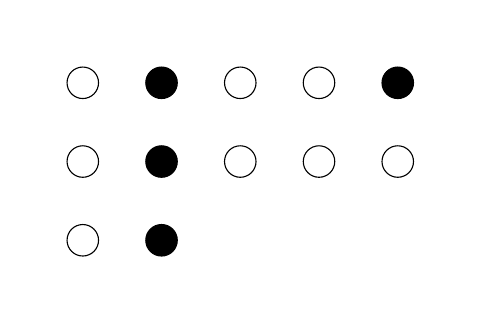
\begin{tikzpicture}[baseline]

    \tikzset{
      point/.style={
        thick,
        draw,
        cross out,
        inner sep=0pt,
        minimum width=5pt,
        minimum height=5pt,
      },
    }
    \clip (-0.7,-2.7) rectangle (4.7,0.7);
    	
	 \filldraw[color={black},fill={white}] (0,0) circle (0.2);
	
	 \filldraw[color={black},fill={black}] (1,0) circle (0.2);
	
	 \filldraw[color={black},fill={white}] (2,0) circle (0.2);
	
	 \filldraw[color={black},fill={white}] (3,0) circle (0.2);
	
	 \filldraw[color={black},fill={black}] (4,0) circle (0.2);
	
	 \filldraw[color={black},fill={white}] (0,-1) circle (0.2);
	
	 \filldraw[color={black},fill={black}] (1,-1) circle (0.2);
	
	 \filldraw[color={black},fill={white}] (2,-1) circle (0.2);
	
	 \filldraw[color={black},fill={white}] (3,-1) circle (0.2);
	
	 \filldraw[color={black},fill={white}] (4,-1) circle (0.2);
	
	 \filldraw[color={black},fill={white}] (0,-2) circle (0.2);
	
	 \filldraw[color={black},fill={black}] (1,-2) circle (0.2);

\end{tikzpicture}\\
	\item Calculer l'expression  $x^2+5x+6$ pour $x=-2$.
	\item Calculer la moyenne de :
            $2\,\,\,; \,\,\,4\,\,\,; \,\,\,28\,\,\,; \,\,\,26$.
	\item $90$ $\%$ de $90= $ $\ldots$
	%\item  $12{,}2$ L $=$ $\ldots$ m$^3$
	\item Développer et réduire l'expression $(5x+1)(4x+2)$.
	\item  Quel est le volume en cm$^3$ de ce  pavé droit ?\\ \begin{tikzpicture}[baseline,scale = 0.8]

    \tikzset{
      point/.style={
        thick,
        draw,
        cross out,
        inner sep=0pt,
        minimum width=5pt,
        minimum height=5pt,
      },
    }
    \clip (-2,-2) rectangle (10,5);
    	\draw[color={black}] (0,0)--(4,0)--(4,3)--(0,3)--cycle;
	\draw[color ={black}, dashed ] (0,0)--(0.87,0.5);
	\draw[color ={black}] (4,0)--(4.87,0.5);
	\draw[color ={black}] (4,3)--(4.87,3.5);
	\draw[color ={black}] (0,3)--(0.87,3.5);
	\draw[color ={black}, dashed ] (0.87,0.5)--(4.87,0.5);
	\draw[color ={black}] (4.87,0.5)--(4.87,3.5);
	\draw[color ={black}] (4.87,3.5)--(0.87,3.5);
	\draw[color ={black}, dashed ] (0.87,3.5)--(0.87,0.5);
	\draw[color ={black},<->] (4,-1)--(0,-1);
	\draw [color={black}] (2,-1.5) node[anchor = center,scale=1, rotate = 0] {4 cm};
	\draw[color ={black},<->] (-1,0)--(-1,3);
	\draw [color={black}] (-1.5,1.5) node[anchor = center,scale=1, rotate = -90] {3 cm};
	\draw[color ={black},>-<] (5.37,-0.37)--(4.5,-0.87);
	\draw [color={black}] (5.19,-1.05) node[anchor = center,scale=1, rotate = -330.11347] {2 cm};

\end{tikzpicture}\\
	\item Pour tout entier naturel $n$, \\
              $\begin{cases} u_0=1\\u_{n+1}=2\times u_n \end{cases}$\,\,\,\,\,\,\,\,\,\,\,\,\,\,\,
              $u_{3}=$  $\ldots$
	\item $7$ $\mu$m $=$ ..... cm
	\item Quelle est l’abscisse  du point $B$ ?\\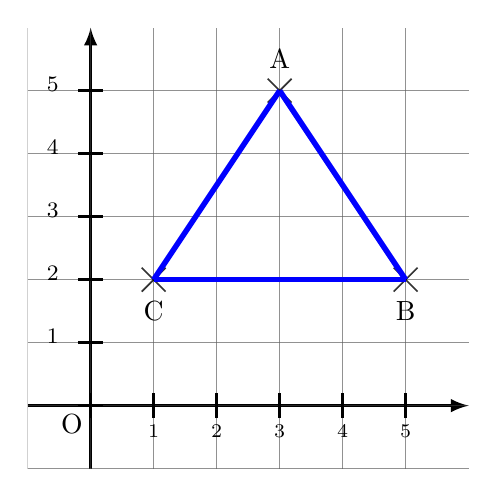
\begin{tikzpicture}[baseline,scale = 0.8]

    \tikzset{
      point/.style={
        thick,
        draw,
        cross out,
        inner sep=0pt,
        minimum width=5pt,
        minimum height=5pt,
      },
    }
    \clip (-1,-1) rectangle (6.1,6);
    	\draw[color ={black},line width = 1.2,>=latex,->] (-1,0)--(6,0);
	\draw[color ={black},line width = 1.2,>=latex,->] (0,-1)--(0,6);
	\draw[color ={black},opacity = 0.4] (-1,1)--(6,1);
	\draw[color ={black},opacity = 0.4] (-1,-1)--(6,-1);
	\draw[color ={black},opacity = 0.4] (-1,2)--(6,2);
	\draw[color ={black},opacity = 0.4] (-1,3)--(6,3);
	\draw[color ={black},opacity = 0.4] (-1,4)--(6,4);
	\draw[color ={black},opacity = 0.4] (-1,5)--(6,5);
	\draw[color ={black},opacity = 0.4] (1,-1)--(1,6);
	\draw[color ={black},opacity = 0.4] (-1,-1)--(-1,6);
	\draw[color ={black},opacity = 0.4] (2,-1)--(2,6);
	\draw[color ={black},opacity = 0.4] (3,-1)--(3,6);
	\draw[color ={black},opacity = 0.4] (4,-1)--(4,6);
	\draw[color ={black},opacity = 0.4] (5,-1)--(5,6);
	\draw[color ={gray},opacity = 0.3] (-1,0)--(6,0);
	\draw[color ={gray},opacity = 0.3] (-1,1)--(6,1);
	\draw[color ={gray},opacity = 0.3] (-1,-1)--(6,-1);
	\draw[color ={gray},opacity = 0.3] (-1,2)--(6,2);
	\draw[color ={gray},opacity = 0.3] (-1,3)--(6,3);
	\draw[color ={gray},opacity = 0.3] (-1,4)--(6,4);
	\draw[color ={gray},opacity = 0.3] (-1,5)--(6,5);
	\draw[color ={gray},opacity = 0.3] (0,-1)--(0,6);
	\draw[color ={gray},opacity = 0.3] (1,-1)--(1,6);
	\draw[color ={gray},opacity = 0.3] (-1,-1)--(-1,6);
	\draw[color ={gray},opacity = 0.3] (2,-1)--(2,6);
	\draw[color ={gray},opacity = 0.3] (3,-1)--(3,6);
	\draw[color ={gray},opacity = 0.3] (4,-1)--(4,6);
	\draw[color ={gray},opacity = 0.3] (5,-1)--(5,6);
	\draw[color ={black},line width = 1.2] (0,-0.2)--(0,0.2);
	\draw[color ={black},line width = 1.2] (1,-0.2)--(1,0.2);
	\draw[color ={black},line width = 1.2] (2,-0.2)--(2,0.2);
	\draw[color ={black},line width = 1.2] (3,-0.2)--(3,0.2);
	\draw[color ={black},line width = 1.2] (4,-0.2)--(4,0.2);
	\draw[color ={black},line width = 1.2] (5,-0.2)--(5,0.2);
	\draw[color ={black},line width = 1.2] (-0.2,0)--(0.2,0);
	\draw[color ={black},line width = 1.2] (-0.2,1)--(0.2,1);
	\draw[color ={black},line width = 1.2] (-0.2,2)--(0.2,2);
	\draw[color ={black},line width = 1.2] (-0.2,3)--(0.2,3);
	\draw[color ={black},line width = 1.2] (-0.2,4)--(0.2,4);
	\draw[color ={black},line width = 1.2] (-0.2,5)--(0.2,5);
	\draw (1,-0.4) node[anchor = center, rotate=0] {\scriptsize \color{black}{$1$}};
	\draw (2,-0.4) node[anchor = center, rotate=0] {\scriptsize \color{black}{$2$}};
	\draw (3,-0.4) node[anchor = center, rotate=0] {\scriptsize \color{black}{$3$}};
	\draw (4,-0.4) node[anchor = center, rotate=0] {\scriptsize \color{black}{$4$}};
	\draw (5,-0.4) node[anchor = center, rotate=0] {\scriptsize \color{black}{$5$}};
	\draw (-0.6,1.1) node[anchor = center, rotate=0] {\footnotesize \color{black}{$1$}};
	\draw (-0.6,2.1) node[anchor = center, rotate=0] {\footnotesize \color{black}{$2$}};
	\draw (-0.6,3.1) node[anchor = center, rotate=0] {\footnotesize \color{black}{$3$}};
	\draw (-0.6,4.1) node[anchor = center, rotate=0] {\footnotesize \color{black}{$4$}};
	\draw (-0.6,5.1) node[anchor = center, rotate=0] {\footnotesize \color{black}{$5$}};
	\draw [color={black}] (-0.3,-0.3) node[anchor = center,scale=1, rotate = 0] {O};
	\draw[color ={black},line width = 0.625,opacity = 0.8] (2.81,5.19)--(3.19,4.81);\draw[color ={black},line width = 0.625,opacity = 0.8] (2.81,4.81)--(3.19,5.19);
	\draw[color ={black},line width = 0.625,opacity = 0.8] (4.81,2.19)--(5.19,1.81);\draw[color ={black},line width = 0.625,opacity = 0.8] (4.81,1.81)--(5.19,2.19);
	\draw[color ={black},line width = 0.625,opacity = 0.8] (0.81,2.19)--(1.19,1.81);\draw[color ={black},line width = 0.625,opacity = 0.8] (0.81,1.81)--(1.19,2.19);
	\draw [color={black}] (3,5.5) node[anchor = center,scale=1, rotate = 0] {A};
	\draw [color={black}] (5,1.5) node[anchor = center,scale=1, rotate = 0] {B};
	\draw [color={black}] (1,1.5) node[anchor = center,scale=1, rotate = 0] {C};
	\draw[color ={blue},line width = 2] (3,5)--(5,2);
	\draw[color ={blue},line width = 2] (3,5)--(1,2);
	\draw[color ={blue},line width = 2] (5,2)--(1,2);

\end{tikzpicture}\\
	\item Donner l'arrondi au centième de $5{,}452\,163$.
          
	\item Soit $(u_n)$ une suite définie pour tout  $n\in\mathbb{N}$ par : $u_n = 7n+4$.\\ $u_{6}=$ $\ldots$
	%\item Si l'on parcourt $30$ km en quinze minutes, alors la vitesse moyenne est :  $\ldots$ km/h
	\item On applique un coefficient multiplicateur de $0{,}24$.\\
          À quelle baisse, en pourcentage, cela correspond-il ? $\ldots$ $\%$
	\item $3{,}1$ h $=$ ..... h ..... min
	\item On donne la courbe représentative d'une fonction $f$. \\
            $f(-1)\times f(1)=$  $\ldots$\\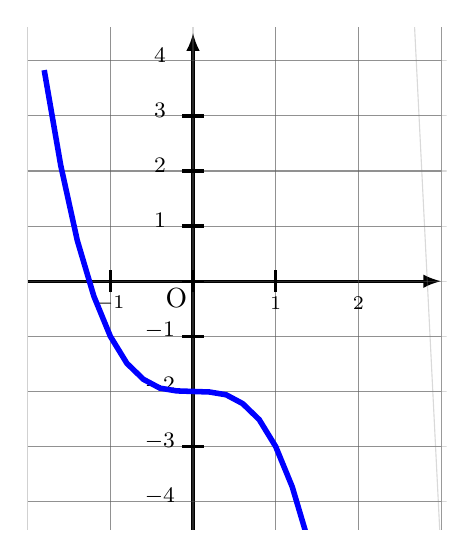
\begin{tikzpicture}[baseline,scale = 0.7]

    \tikzset{
      point/.style={
        thick,
        draw,
        cross out,
        inner sep=0pt,
        minimum width=5pt,
        minimum height=5pt,
      },
    }
    \clip (-3,-4.5) rectangle (4.6,4.6);
    	\draw[color ={black},line width = 1.2,>=latex,->] (-3,0)--(4.5,0);
	\draw[color ={black},line width = 1.2,>=latex,->] (0,-5)--(0,4.5);
	\draw[color ={black},opacity = 0.4] (-3,1)--(4.5,1);
	\draw[color ={black},opacity = 0.4] (-3,-1)--(4.5,-1);
	\draw[color ={black},opacity = 0.4] (-3,2)--(4.5,2);
	\draw[color ={black},opacity = 0.4] (-3,-2)--(4.5,-2);
	\draw[color ={black},opacity = 0.4] (-3,3)--(4.5,3);
	\draw[color ={black},opacity = 0.4] (-3,-3)--(4.5,-3);
	\draw[color ={black},opacity = 0.4] (-3,4)--(4.5,4);
	\draw[color ={black},opacity = 0.4] (-3,-4)--(4.5,-4);
	\draw[color ={black},opacity = 0.4] (1.5,-5)--(1.5,5); %
	\draw[color ={black},opacity = 0.4] (-1.5,-5)--(-1.5,5); %
	%\draw[color ={black},opacity = 0.4] (2,-5)--(2,5);
	%\draw[color ={black},opacity = 0.4] (-2,-5)--(-2,5);
	\draw[color ={black},opacity = 0.4] (3,-5)--(3,5);
	\draw[color ={black},opacity = 0.4] (-3,-5)--(-3,5);
	\draw[color ={black},opacity = 0.4] (4.5,-5)--(4.5,5); %
	\draw[color ={gray},opacity = 0.3] (-3,0)--(7.5,0);
	\draw[color ={gray},opacity = 0.3] (-3,1)--(7.5,1);
	\draw[color ={gray},opacity = 0.3] (-3,-1)--(7.5,-1);
	\draw[color ={gray},opacity = 0.3] (-3,2)--(7.5,2);
	\draw[color ={gray},opacity = 0.3] (-3,-2)--(7.5,-2);
	\draw[color ={gray},opacity = 0.3] (-3,3)--(7.5,3);
	\draw[color ={gray},opacity = 0.3] (-3,-3)--(7.5,-3);
	\draw[color ={gray},opacity = 0.3] (-3,4)--(7.5,4);
	\draw[color ={gray},opacity = 0.3] (-3,-4)--(7.5,-4);
	\draw[color ={gray},opacity = 0.3] (0,-5)--(0,5);
	\draw[color ={gray},opacity = 0.3] (1.5,-5)--(1.5,5); %
	\draw[color ={gray},opacity = 0.3] (-1.5,-5)--(-1.5,5); %
	%\draw[color ={gray},opacity = 0.3] (2,-5)--(2,5);
	%\draw[color ={gray},opacity = 0.3] (-2,-5)--(-2,5);
	\draw[color ={gray},opacity = 0.3] (3,-5)--(3,5);
	\draw[color ={gray},opacity = 0.3] (-3,-5)--(-3,5);
	\draw[color ={gray},opacity = 0.3] (4.5,-5)--(4,5); %
	%\draw[color ={gray},opacity = 0.3] (5,-5)--(5,5);
	\draw[color ={gray},opacity = 0.3] (6,-5)--(6,5);
	\draw[color ={gray},opacity = 0.3] (7,-5)--(7,5);
	\draw[color ={black},line width = 1.2] (0,-0.2)--(0,0.2);
	\draw[color ={black},line width = 1.2] (1.5,-0.2)--(1.5,0.2);
	\draw[color ={black},line width = 1.2] (-1.5,-0.2)--(-1.5,0.2);
	\draw[color ={black},line width = 1.2] (-0.2,0)--(0.2,0);
	\draw[color ={black},line width = 1.2] (-0.2,1)--(0.2,1);
	\draw[color ={black},line width = 1.2] (-0.2,-1)--(0.2,-1);
	\draw[color ={black},line width = 1.2] (-0.2,2)--(0.2,2);
	\draw[color ={black},line width = 1.2] (-0.2,-2)--(0.2,-2);
	\draw[color ={black},line width = 1.2] (-0.2,3)--(0.2,3);
	\draw[color ={black},line width = 1.2] (-0.2,-3)--(0.2,-3);
	\draw (1.5,-0.4) node[anchor = center, rotate=0] {\scriptsize \color{black}{$1$}};
	\draw (3,-0.4) node[anchor = center, rotate=0] {\scriptsize \color{black}{$2$}};
	\draw (-1.5,-0.4) node[anchor = center, rotate=0] {\scriptsize \color{black}{$-1$}};
	\draw (-0.6,1.1) node[anchor = center, rotate=0] {\footnotesize \color{black}{$1$}};
	\draw (-0.6,2.1) node[anchor = center, rotate=0] {\footnotesize \color{black}{$2$}};
	\draw (-0.6,3.1) node[anchor = center, rotate=0] {\footnotesize \color{black}{$3$}};
	\draw (-0.6,4.1) node[anchor = center, rotate=0] {\footnotesize \color{black}{$4$}};
	\draw (-0.6,-0.9) node[anchor = center, rotate=0] {\footnotesize \color{black}{$-1$}};
	\draw (-0.6,-1.9) node[anchor = center, rotate=0] {\footnotesize \color{black}{$-2$}};
	\draw (-0.6,-2.9) node[anchor = center, rotate=0] {\footnotesize \color{black}{$-3$}};
	\draw (-0.6,-3.9) node[anchor = center, rotate=0] {\footnotesize \color{black}{$-4$}};
	\draw [color={black}] (-0.3,-0.3) node[anchor = center,scale=1, rotate = 0] {O};
	\draw[color={blue},line width = 2] (-2.7,3.83)--(-2.4,2.1)--(-2.1,0.74)--(-1.8,-0.27)--(-1.5,-1)--(-1.2,-1.49)--(-0.9,-1.78)--(-0.6,-1.94)--(-0.3,-1.99)--(0,-2)--(0.3,-2.01)--(0.6,-2.06)--(0.9,-2.22)--(1.2,-2.51)--(1.5,-3)--(1.8,-3.73)--(2.1,-4.74);

\end{tikzpicture}\\
	\item $f(x)=3x^2+2x-1$.\\
          $f'(x)=$  $\ldots$


\end{enumerate}
\vfill\null
\columnbreak
\textcolor{UGLiBlue}{
    Jeudi 13/03/2025\\
    NOM, Prénom :}\\

\end{multicols}
\newpage

\begin{multicols}{2}
	\classe{\terminale Comp}
    \titre{\includegraphics[width=3cm]{CAN.png} Corrigé interro 2}
    \maketitle
\begin{enumerate}[itemsep=.75em]
    \item $9 \times 0{,}4=9\times 4\times 0,1=3{,}6$
\item $3-\dfrac{2}{3}= \dfrac{9}{3}-\dfrac{2}{3}=\dfrac{7}{3}$
\item $5\times10^2+5+6\times 10^{-1}=500+5+0{,}6=505{,}6$
\item On se ramène à une équation du type $a\times x=b$ :\\
          $\begin{aligned}
          3x+6&=0\\
         3x&=-6\\
                              x&=\dfrac{-6}{3}=-\dfrac{2{\color[HTML]{2563a5}\boldsymbol{\times3}} }{1{\color[HTML]{2563a5}\boldsymbol{\times3}}}=-2
         \end{aligned}$\\
          
        
          
          L'équation $3x+6=0$ a pour solution $x=-2$.
\item $4$ croissants coûtent  $3{,}60$ €, donc
                       $2$ croissants coûtent $2$ fois moins, soit : \\
                       $3{,}60\div 2=1{,}80$ €.
\item La fréquence est donnée par le quotient : $\dfrac{\text{Nombre de boules noires}}{\text{Nombre total de boules}}=\dfrac{4}{12}=\dfrac{1{\color[HTML]{2563a5}\boldsymbol{\times4}} }{3{\color[HTML]{2563a5}\boldsymbol{\times4}}}=\dfrac{1}{3}$.
\item 
            Pour $x=-2$, on obtient : $x^2+5x+6=(-2)^2+5\times (-2)+6=0$.
                      
\item La moyenne est donnée par : $\dfrac{2+4+28+26}{4}=\dfrac{60}{4}=15$.
\item           Prendre $90$ $\%$  de $90$ revient à prendre $9\times 10$ $\%$  de $90$.\\
            Comme $10$ $\%$  de $90$ vaut $9$ (pour prendre $10$ $\%$  d'une quantité, on la divise par $10$), alors
            $90$ $\%$ de $90=9\times 9=81$.
           
%\item Comme $1$ L= $0,001$ m$^3$, $12{,}2$ L $=0{,}012\,2$  m$^3$.
\item $(5x+1)(4x+2)=20x^2+10x+4x+2=20x^2+14x+2$
\item Le volume de ce pavé droit est : $4\times 3\times 2=24$ cm$^3$.
\item On calcule les termes avc la formule de récurrence :\\ $u_{1} = {\color{violet}\boldsymbol{ u_{0}}} \times 2 =
                    {\color{violet}\boldsymbol{1}} \times 2 = {\color{purple}\boldsymbol{2}}$\\ $u_{2} = {\color{purple}\boldsymbol{ u_{1}}} \times 2 =
                    {\color{purple}\boldsymbol{2}} \times 2 = {\color{blue}\boldsymbol{4}}$\\ $u_{3} = {\color{blue}\boldsymbol{ u_{2}}} \times 2 =
                    {\color{blue}\boldsymbol{4}} \times 2 = {\color[HTML]{008002}\boldsymbol{8}}$
\item $1$ $\mu$m $=10^{-6}$ m, donc $1$ $\mu$m  $=10^{-4}$ cm  $=0{,}000\,1$ cm.\\
            Ainsi, $7$ $\mu$m $=0{,}000\,7$ cm.
\item L'abscisse du point $B$ se lit sur l'axe horizontal. \\
            $x_B=5$.
            
\item Le chiffre qui suit les centièmes est $2<5$, donc l'arrondi au centième de $5{,}452\,163$ est $5{,}45$.
\item Dans l'expression de $u_n$ on remplace $n$ par $6$, on obtient : $u_{6} =7 \times 6 +4=46$.
%\item Quinze minutes représentent $\dfrac{1}{4}$ heure.\\
%          Donc en $1$ heure, on parcourt $30\times 4=120$ km. \\
%          La vitesse moyenne est donc $120$ km/h. 
\item Multiplier par $0{,}24$ revient à multiplier par $1-\dfrac{76}{100}$. \\
          Cela revient donc à baisser de $76 \%$. 
\item $3{,}1$ h $ = 3$ h $ + 0{,}1 \times 60$ min $  = 3$ h $6$ min
\item $f(-1)=-1$ et $f(1)=-3$, donc $f(-1)\times f(1)=-1\times (-3)=3$.
\item $f(x)=3x^2+2x-1$.\\
          $f'(x)=6x+2$.
\end{enumerate}
\end{multicols}
\end{document}